\chapter{Podaci i metode binarne klasifikacije} % Main chapter title
\label{Chapter3}

U ovom poglavlju biće opisani korišćeni podaci i način njihovog predstavljanja u račnuaru. Zatim će ukratko biti opisane metode binarne klasifikacije koje su korišćene za predviđanje funkcija proteina.


\section{Podaci}

Podaci o proteinima mogu se pronaći u biomedicinskim bazama podataka, a neke od njih prikazane su u tabeli \ref{tab: databases}. 

\begin{table}[H]
	\centering
	\begin{tabular}{|l|l|l|}
		\hline
		Baza podataka & URL & Opis \\
		\hline
		UniProtKB & \url{uniprot.org} & Proteinske sekvence i \\ & & funkcije proteina \\
		\hline
		PFAM & \url{pfam.xfam.org} & Proteinske familije \\
		\hline
		PDB & \url{wwpdb.org} & Eksperimentalno utvrđene strukture \\
		\hline
		ModBase & \url{modbase.compbio.ucsf.edu} & Strukture utvrđene predviđanjem \\
		\hline
		I2D & \url{ophid.utoronto.ca} & Interakcije između proteina \\
		\hline
		GEO & \url{www.ncbi.nlm.nih.gov/geo} & Podaci o genskoj ekspresiji \\
		\hline
		PRIDE & \url{www.ebi.ac.uk/pride} & Podaci dobijeni \\
		& & masenom sprektometrijom \\
		\hline 
	\end{tabular}
	\caption{Prikaz nekih javno dostupnih biomedicinskih baza \\ podataka \cite{radivojac, doktJK}.}
	\label{tab: databases}
\end{table}



\subsection{Predstavljanje proteina}

% predstavljanje proteina preko sekvenci aminokiselina

Kao što je već rečeno, proteini su izgrađeni od 20 različitih aminokiselina, a svaka aminokiselina ima jedinstveni simbol (tabela \ref{tab: aminoacids}). Najjednostavniji način za predstavljanje proteina u računaru jeste kao niska karaktera nad azbukom $\Sigma = \{A, C, D, E, F,$ \\ $ G, H, I, K, L, M, N, P, Q, R, S, T, V, W, Y\}$. Nad ovako predstavljenim proteinima mogu su koristiti algoritmi za rad sa tekstom kao što je poravnanje sekvenci \cite{radivojac}.


\subsection{Predstavljanje funkcije proteina}

Da bi predviđanje funkcija proteina bilo moguće neophodno je da postoje dobro definisani odnosi između funkcija. Sistem za predstavljanje funkcije proteina koji se trenutno najviše koristi je \textit{Gene Ontology}. Ovaj sistem deli funkcije proteina na tri ontologije: biološki procesi (BPO), molekulske funkcije (MFO) i ćelijske komponente (CCO). 


Svaka ontologija predstavljena je kao usmereni aciklički graf gde su čvorovima pridruženi nazivi funkcija, a grane koje ih povezuju definišu relaciju ‚‚is\_a''. Hijerarhijska organizacija obezbeđuje da svaki čvor ima specifičniju funkciju od roditeljskog čvora. U ovoj hijerarhiji jedan čvor može imati više roditeljskih čvorova što je prikazano na slici \ref{fig:subgraph} \cite{doktJK, GO}. U korenu svake ontologije nalazi se funkcija sa nazivom te ontologije, a u listovima su najspecifičnije fukcije.


\begin{figure}[h]
	\centering
	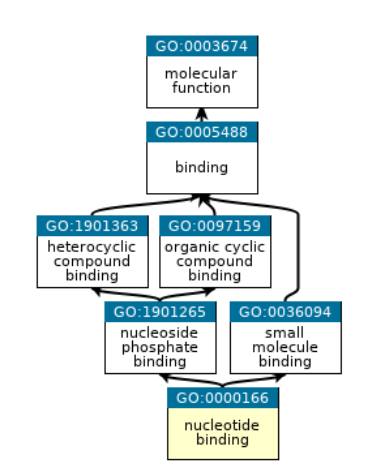
\includegraphics[width=0.6\textwidth]{Figures/go_subgraph.png}
	\caption{Prikaz svih predaka lista označenog funkcijom ‚‚nucleotid binding'' u ontologiji molekulskih funkcija.}
	\label{fig:subgraph}
\end{figure}


\section{Binarni klasifikatori}

Klasifikacija, odnosno, zadatak dodeljivanja objekata jednoj od više predefinisanih kategorija, rasprostranjen je problem koji obuhvata mnoštvo različitih primena. Primeri uključuju otkrivanje spam poruka na osnovu zaglavlja poruke i njenog sadržaja, kategorisanje ćelija kao malignih ili beningnih na osnovu rezultata magnetne rezonance, klasifikaciju galaksija na osnovu njihovog oblika, itd. Binarna klasifikacija je slučaj klasifikacije u kojoj postoje tačno dve predefinisane kategorije u koje treba razvrstati date objekte. Obično se za jednu kategoriju kaže da je to pozitivna klasa, a za drugu da je negativna.

Svaki klasifikator upotrebljava algoritam za učenje kako bi odredio model koji najbolje odgovara vezi između skupa atributa i klase ulaznih podataka. Model koji algoritam generiše trebalo bi da odgovara ulaznim podacima kao i da tačno predviđa klasu slogova koje ranije nije video. 


\subsection{Metod potpornih vektora} 

Metod potpornih vektora (engl. \textit{support vector machine}) je tehnika za klasifikaciju zasnovana na ideji vektorskih prostora. Ova metoda generiše klasifikacioni model koji predstavlja funkciju. Osnovni algoritam definisan je za binarnu klasifikaciju.

Osnovna ideja ove metode jeste pronalazak razdvajajuće hiperravni takve da su instance iste klase sa iste strane ravni. Sa tako postavljenim uslovom, razdvajajućih hiperravni može biti više od jedne što je prikazano na slici \ref{fig:svm1}. Iako svaka od ravni razdvaja podatke bez greške, nema garancije da će se podjednako dobro ponašati sa novim podacima koje je potrebno klasifikovati. 


\begin{figure}[H]
	\centering
	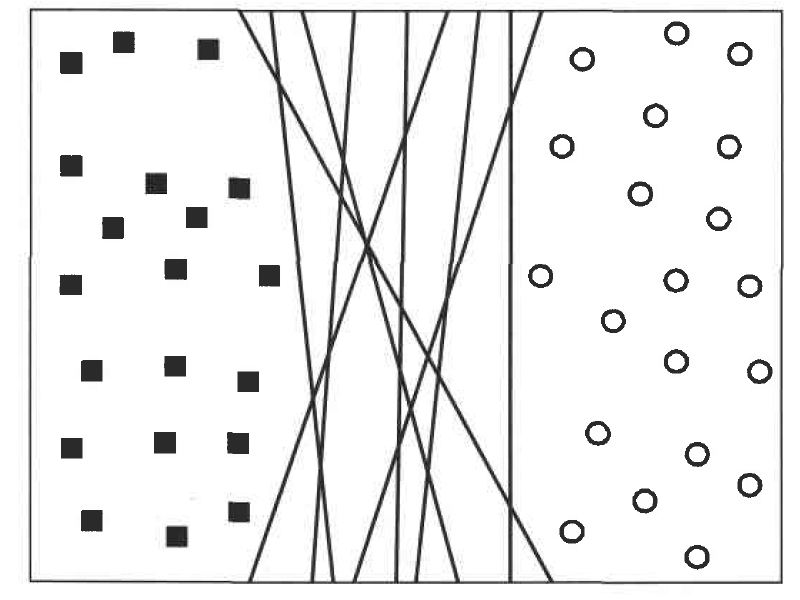
\includegraphics[width=0.6\textwidth]{Figures/svm1.png}
	\caption{Primeri razdvajajućih hiperravni \cite{introDM}}
	\label{fig:svm1}
\end{figure}


Na slici \ref{fig:svm2} izdvojene su dve hiperravni $B_1$ i $B_2$ i za svaku su dodate dve pomoćne hiperavni $b_{i1}$ i $b_{i2}$. Pomoćne ravni paralelne su glavnoj i pomerene u levu ili desnu stranu do najbliže instance jedne klase. Rastojanje između pomoćnih ravni odnosno rastojanje između najbližih instanci iz obe klase u odnosu na hiperravan naziva se \textit{margina}, a  instance oslonjene na hiperravni su \textit{potporni vektori}. Cilj je pronaći hiperravan koja maksimizuje veličinu margine. Sa slike \ref{fig:svm2} jasno se vidi da je bolja hiperravan $B_1$. Jednačina optimalne hiperravni predstavlja klasifikacioni model. Korak klasifikacije nepoznate instance sastoji se iz izračunavanja njenog rastojanja od hiperravni na osnovu čega se određuje klasa kojoj instanca pripada \cite{introDM, doktJG}.



\begin{figure}[h]
	\centering
	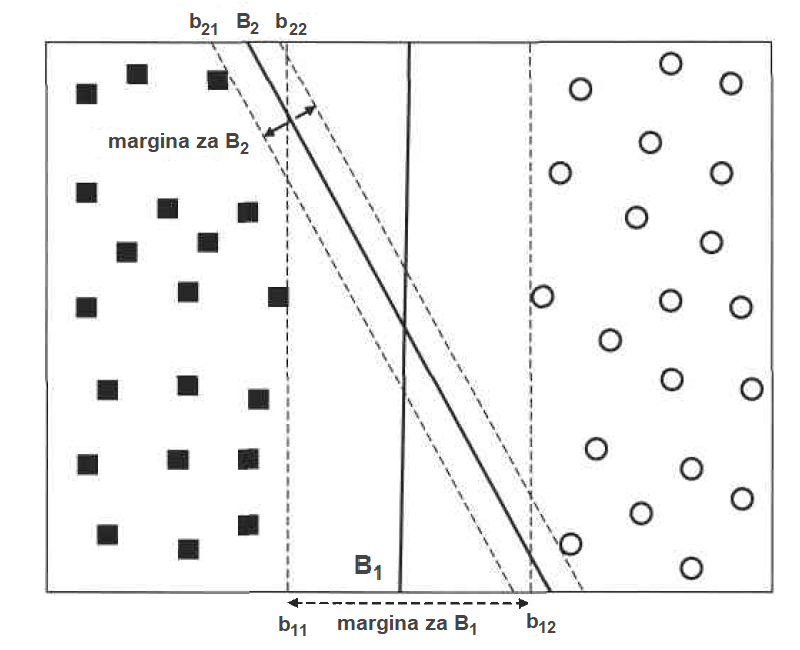
\includegraphics[width=0.6\textwidth]{Figures/svm2.png}
	\caption{Margine razdvajajućih hiperravni \cite{introDM}}
	\label{fig:svm2}
\end{figure}


Jednačina hiperravni je

$$w \cdot x + w_0 = 0$$

\noindent gde je $w_0$ slobodan član. Na osnovu jednačine rastojanja tačke od hiperravni

$$\dfrac{|w \cdot x + w_0|}{||w||_2}$$

\noindent i činjenice da za svaku od tačaka sa ovih hiperravni važi $w \cdot x + w_0 = 1$, dobija se da je ukupno rastojanje između klasa, u pravcu normalnom u odnosu na optimalnu hiperravan $\dfrac{2}{|w|}$. Tako se optimalna hiperravan dobija pronalaženjem koeficijenata koji maksimizuju ovaj izraz pod uslovima da su sve tačke sa pravih strana te hiperravni odnosno da su podaci linearno razdvojivi. Optimizacioni problem može da se zapiše i kao problem minimizacije i glasi:

$$ \underset{w, w_0}{min} \dfrac{||w||_2}{2}$$
$$ y_i(w \cdot x_i + w_0) \geq 1 \qquad i=1, \ldots, N $$
 
Dodatni uslov će obezbediti da sve tačke budu na većem rastojanju od hiperravni u odnosu na potporne vektore \cite{ml}.

S obzirom da je čest slučaj da podaci nisu linearno razdvojivi potrebno je prihvatiti greške tj. dozvoliti da se neka instanca nađe sa pogrešne strane razdvajajuće hiperravni. U tu svrhu uvode se nove promenljive, $\xi_i$ koje mere koliko je svaka pogrešno klasifikovana instanca udaljena od hiperravni. Taj metod nazivamo metod potpornih vektora sa \textit{mekom marginom}. Optimizacioni problem se menja:

$$ \underset{w, w_0}{min} \dfrac{||w||_2}{2} + C\sum_{i=0}^{N} \xi_i$$
$$ y_i(w \cdot x_i + w_0) \geq 1 - \xi_i \qquad i=1, \ldots, N $$
$$ \xi_i \geq 0  \qquad i=1, \ldots, N $$
 
Metaparametar $C$ kontroliše koliki značaj imaju greške. Ukoliko je vrednost jednaka nuli, onda greške ne igraju nikakvu ulogu, a ako je vrednost velika, onda su greške veoma važne, a pravac hiperravni i širina pojasa nisu bitne \cite{ml}. 


\subsection{Logistička regresija}

Logistička regresija (engl. \textit{logistic regression}) je statistički zasnovan metod za analizu skupa podataka u kom jedna ili više nezavisnih promenljivih određuju ishod. Osnovna pretpostvaka je Bernulijeva rasporedela ciljne promenljive $y$ pri datim vrednostima atributa $x$ odnosno, za date vrednosti atributa $x$, postoji parametar $\mu \in [0, 1]$ tako da važi:

$$ p(y = 1 | x) = \mu $$ 

\noindent odakle je $ p(y=0 | x)$  jednoznačno određeno.
Zadatak je sličan kao u prethodnoj metodi, potrebno je pronaći razdvajajuću hiperravan koja deli podatke tako da sa jedne strane budu instance iste klase. Najjednostavniji je linearan model:

$$f(x) = w \cdot x$$

S obzirom da funkcija uzima vrednosti iz intervala $[-\infty, \infty]$, a parametar $\mu$ mora imati vrednost iz intervala $[0, 1]$ da bi verovatnoća bila ispravno definisana, ovakav model nije prihvatljiv. Zbog toga se vrednost linearnog modela transformiše monotonom funkcijom u interval $[0, 1]$. U te svrhe, najčešće se koristi sigmoidna funkcija:

$$\sigma(t) = \dfrac{1}{1+exp(-t)}$$

čiji je grafik prikazan na slici \ref{fig:sigmoid}. Nakon transformacije vrednosti linearnog modela sigmoidnom funkcijom, model logističke regresije određen je relacijom:

$$p_w(y = 1 | x) = \sigma(w \cdot x)$$


Iz toga se može odrediti i puna specifikacija problema:

$$p_w(y | x) = \sigma(w \cdot x)^y (1 - \sigma(w \cdot x))^{1-y}$$

Verovatnoća da instanca pripada jednoj klasi je veća što je instanca dalje od hiperravni sa odgovarajuće strane \cite{ml}.

\begin{figure}[h]
	\centering
	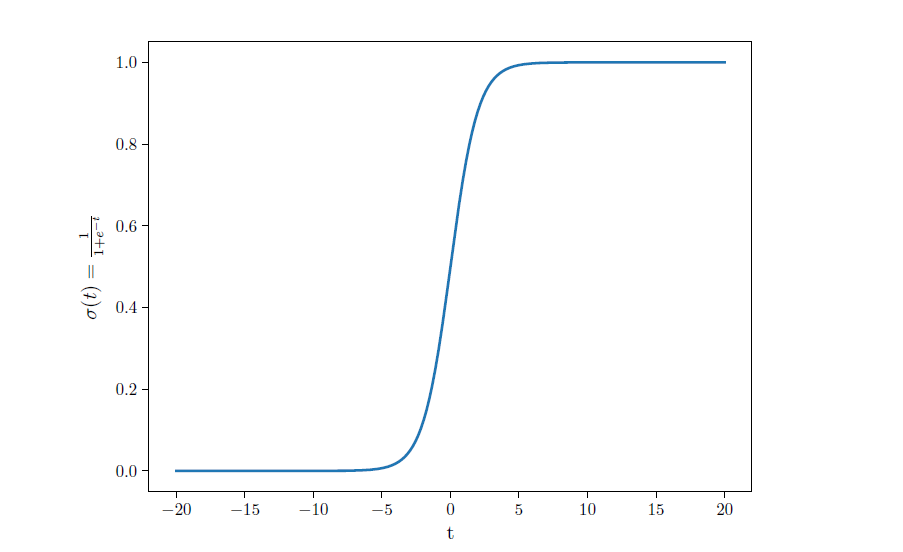
\includegraphics[width=0.8\textwidth]{Figures/sigmoid.png}
	\caption{Grafik sigmoidne funkcije \cite{ml}}
	\label{fig:sigmoid}
\end{figure}

Ocena parametara ovog modela zasniva se na principu maksimalne verodostojnosti. Uz pretpostavku nezavisnosti instanci, funkcija verodostojnosti zadata je izrazom:

$$\mathcal{L}(w) = \prod_{i=1}^{N}p_w(y_i|x_i)$$

i potrebno je rešiti problem:

$$\underset{w}{\text{max }}\mathcal{L}(w)$$

Ukoliko se pređe na negativan logaritam verodostojnosti optimizacioni problem postaje:

$$ \underset{w}{min} -\sum_{i=0}^{N} [y_i\log f_w(x_i) + (1-y_i)\log(1 - f_w(x_i))]$$



\subsection{Slučajne šume} 

Metod slučajne šume (engl. \textit{random forests}) spada u grupu metoda specijalno dizajnirane za stabla odlučivanja. Ona kombinuje predviđanja više različitih stabala, gde je svako stablo generisano na osnovu vrednosti nezavisnog skupa slučajno odabranih vektora.

\subsubsection{Stabla odlučivanja}
 
Problem klasifikacije rešava se postavljanjem pažljivo sastavljenih pitanja o atributima podataka. Pitanja se postavljaju sve dok nije moguće zaključiti klasu date instance. Niz pitanja i odgovora organizovan je u hijerarhijsku strukturu koja se sastoji iz čvorova i direktinih grana. Na slici \ref{fig:tree} je prikazano stablo odlučivanja koje određuje da li je životinja opasna ili ne na osnovu podataka o otrovnosti, veličini i ishrani. 

Svaki list u stablu ima dodeljenu klasu, a unutrašnji čvorovi i koren sadrže uslove koji razdvajaju instance sa različitim karakteristikama. Grane predstavljaju odgovor na pitanje čvora iz kog izlaze. Jednom kada je stablo konstruisano, klasifikacija je jednosmerna. Kreće se od korenog čvora i za konkretnu instancu odgovara se na pitanja koja se nalaze u čvorovima praćenjem odgovarajućih grana sve do listova koje sadrže konačan odgovor. Klasa koja je pridružena listu dodeljuje se instanci \cite{introDM}.


\begin{figure}[h]
	\centering
	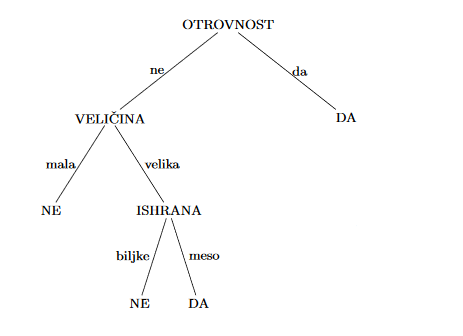
\includegraphics[width=0.7\textwidth]{Figures/tree.png}
	\caption{Primer stabla odlučivanja koje određuje da li je životinja opasna ili ne \cite{vi}}
	\label{fig:tree}
\end{figure}



\subsubsection{Predviđanje korišćenjem slučajnih šuma} 


Osnovna ideja je kombinovanje više stabala odlučivanja u jedan model. Stabla koja se kombinuju treniraju se nad nezavisnim, slučajno odabranim podskupovima podataka, a može se koristiti i slučajno odabran podskup atributa. Obučavaju se nad različitim skupovima kako bi njihove greške bile što slabije korelisane \cite{ml}.  
 
Instanca se klasifikuje glasanjem. Svako od konstruisanih stabala klasifikuje instancu u jednu od dve klase, a zatim se svi odgovori broje i odgovor klasifikatora slučajne šume je ona klasa koja ima više glasova tj. ona klasa koju je više stabala predvidelo. Slika \ref{fig:rf} ilustruje proces treniranja i klasifikacije.


\begin{figure}[H]
	\centering
	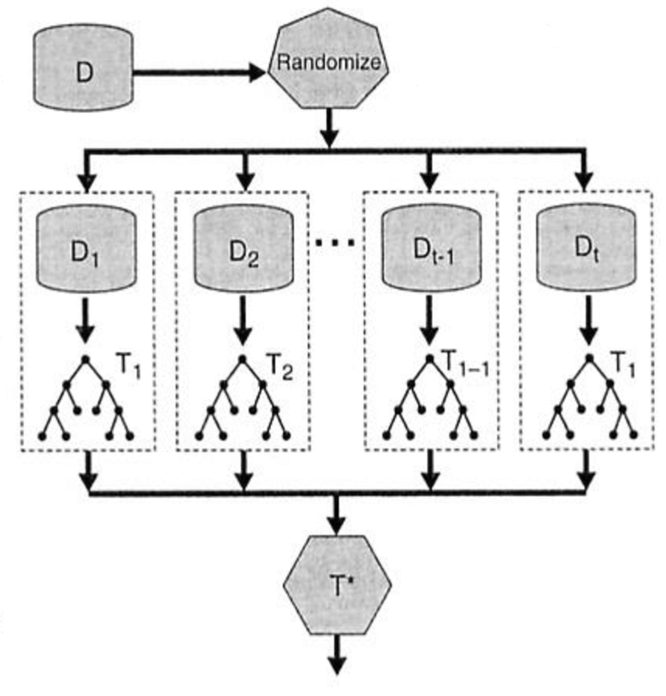
\includegraphics[width=0.6\textwidth]{Figures/random_forests.png}
	\caption{Primer slučajne šume \cite{introDM}. Prvo se iz početnog skupa slučajno odabiraju instance i formira se podskup za svako stablo. Zatim se nad odgovarajućim podskupovima treniraju stabla. Svako stablo klasifikuje nepoznatu instancu i odgovori se kombinuju u jedan, konačan, odgovor modela slučajnih šuma.}
	\label{fig:rf}
\end{figure}



\section{Evaluacija modela binarne klasifikacije}
\label{sec:evaluation}

Metode binarne klasifikacije za test instancu daju jedan od dva moguća odgovora, na primer, ‚‚da'' ili ‚‚ne''. Pošto se jedna klasa obično posmatra kao pozitivna a druga kao negativna, neka u ovom primeru ‚‚da'' bude pozitivna klasa, a ‚‚ne'' neka bude negativna klasa. Prilikom ocenjivanja kvaliteta klasifikacionog modela od značaja su 4 veličine:

\begin{itemize}
	\item $tp$ - broj instanci za koju je predviđena pozitivna klasa i čija je stvarna klasa pozitivna
	
	\item $tn$ - broj instanci za koju je predviđena negativna klasa i čija je stvarna klasa negativna
	
	\item $fp$  - broj instanci za koju je predviđena pozitivna klasa, a čija je stvarna klasa negativna
	
	\item $fn$ - broj instanci za koju je predviđena negativna klasa, a čija je stvarna klasa pozitivna.
	
\end{itemize}


Kada su definisane ove veličine, mogu se odrediti i neke mere kvaliteta. Na primer, tačnost modela. Tačnost (\textit{engl. accuracy}) određuje koliko je instanci tačno klasifikovano u odnosu na ukupan broj instanci i definiše se formulom:

$$\text{accuracy = } \dfrac{tp + tn}{tp +tn +fp +fn}$$ 

Ova metrika se često koristi u mašinskom učenju, međutim, ona ne daje uvek dobru ocenu metoda. U slučaju nebalansiranih klasa\footnote{Pod nebalansiranim klasama podrazumeva se da u skupu podataka postoji mnogo više instanci koji pripadaju jednoj klasi u odnosu na broj instanci koje pripadaju drugoj klasi.} model može da daje visoku vrednost za tačnost, a da ipak loše predviđa. Razlog je to što često loši modeli predviđaju skoro uvek samo jednu, dominantnu klasu, a pošto je instanci dominantne klase značajno više, većina instanci će biti ispravno klasifikovana. Međutim, cilj je napraviti model koji će biti uspešan u klasifikovanju obe klase, a ne samo jedne \cite{f1}.

Zbog toga se definišu još neke mere kvaliteta modela. Prva je preciznost (\textit{engl. precision}), a druga je odziv (\textit{engl. recall}) i definišu se formulama:

$$ \text{precision = } \dfrac{tp}{tp + fp}  \qquad  \qquad \text{recall = } \dfrac{tp}{tp + fn}$$

\noindent Preciznost određuje koliko je pozitivnih instanci ispravno klasifikovano u odnosu na ukupan broj instanci koje su klasifikovane kao pozitivne. Sa druge strane, odziv određuje udeo ispravno klasifikovanih pozitivnih instanci u odnosu na ukupan broj pozitivnih instanci u skupu. 

Preciznost i odziv pojedinačno nisu korisne. Ukoliko su sve instance klasifikovane kao pozitivne, odziv će biti maksimalan, međutim preciznost će biti katastrofalna, dok sa druge strane, ukoliko su sve instance klasifikovane kao negativne model ne greši i preciznost je maksimalna, ali odziv je veoma loš. Stoga ima smisla posmatrati ih zajedno što se često radi određivanjem njihove harmoniske sredine koja je nazvana $f_1$-mera \cite{ml}:

$$f_1 = 2 \cdot \dfrac{\text{precision} \cdot \text{recall}}{\text{precision} + \text{recall}}$$


